\documentclass[11pt]{article}

% ---------- Page layout ----------
\usepackage[margin=1in]{geometry}
\usepackage{setspace}
\onehalfspacing

% ---------- Math ----------
\usepackage{amsmath,amssymb,amsfonts}
\usepackage{bm}
\usepackage{mathtools}

% ---------- Figures and tables ----------
\usepackage{graphicx}
\usepackage{booktabs}
\usepackage{multirow}
\usepackage{subcaption}
\usepackage{float}

% ---------- Algorithms ----------
\usepackage{algorithm}
\usepackage{algorithmic}

% ---------- References ----------
\usepackage[colorlinks=true,linkcolor=blue,citecolor=blue,urlcolor=blue]{hyperref}
\usepackage{cite}

% ---------- Misc ----------
\usepackage{xcolor}

% ---------- Custom commands ----------
\newcommand{\R}{\mathbb{R}}
\newcommand{\C}{\mathbb{C}}
\newcommand{\re}{\mathrm{Re}}
\newcommand{\im}{\mathrm{Im}}
\DeclareMathOperator{\diag}{diag}
\DeclareMathOperator*{\argmin}{arg\,min}
\newcommand{\pd}[2]{\frac{\partial #1}{\partial #2}}

\title{High-Fidelity Differentiable DAE Simulation of\\
Mixed Synchronous-Generator and Inverter-Based\\Power Systems}

\author{
Hamad Alduaij\\
School of Electrical, Computer, and Energy Engineering\\
Arizona State University, Tempe, AZ 85287, USA\\
\texttt{halduaij@asu.edu}
}

\date{}

\begin{document}
\maketitle

\begin{abstract}
Training neural controllers for power systems with high inverter penetration
requires gradient information through the differential-algebraic equations
(DAEs) that govern network dynamics.  Existing simulators solve these DAEs
at high fidelity but provide no gradients; general-purpose autodiff
frameworks lack implicit algebraic constraint solvers.  This paper presents
an open-source, fully differentiable DAE simulator for the IEEE~39-bus
system with both 6-state grid-following (GFL) and 6-state grid-forming
(GFM) inverter models.  The simulator combines analytic Jacobians for the
Newton-based power flow solve with an implicit function theorem (IFT)
backward pass, enabling exact gradient computation at cost comparable to the
forward simulation.  The system model includes two-axis synchronous
generators with AVR and governor-turbine dynamics, ZIP loads on a
Kron-reduced network, PLL-based GFL inverters with algebraic current loops,
and GFM inverters with adaptive virtual inertia behind a virtual impedance.
Both models are cast in control-affine form $\dot{x} = f(x) + g(x)u$ for
structured controller design.  Batched GPU execution supports parallel
trajectory rollouts for reinforcement learning and Monte Carlo studies.
Gradient accuracy is validated against finite differences (relative error
$< 10^{-4}$), simulation fidelity is verified against ANDES, and
computational benchmarks demonstrate [X]$\times$ speedup with GPU batching.
The codebase, including incremental energy functions and Lyapunov
observables for physics-informed training, is released at
\url{https://github.com/halduaij/differentiable-dae-simulator}.

\end{abstract}

% ============================================================================
\section{Introduction}
\label{sec:intro}
% ============================================================================

Power systems with increasing shares of inverter-based resources (IBR)
present new control challenges.  As synchronous generators retire,
system inertia decreases and frequency dynamics become faster and less
predictable~\cite{Milano18LowInertiaReview, NREL21GFMRoadmap}.
Grid-forming (GFM) inverters can restore inertial response through
virtual synchronous generator (VSG)
algorithms~\cite{Zhong11Synchronverters, Bevrani14VSGSurvey}, but
tuning these controllers across heterogeneous operating conditions
remains difficult.  Data-driven methods, including reinforcement
learning and neural Lyapunov
approaches~\cite{CuiZhang23Lyapunov, Shuai25SafeRL, Feng24VariableInertia},
have shown promise for this task.  These methods require
gradient information through the system dynamics to update controller
parameters during training.

Computing gradients through power system dynamics is complicated by the
differential-algebraic equation (DAE) structure.  The differential
states (generator angles, frequencies, inverter internal variables)
evolve continuously, while the algebraic states (bus voltages and
angles) are determined at each instant by the implicit power flow
equations.  A Newton-based solver finds the algebraic states, creating
a nondifferentiable bottleneck: standard automatic differentiation
cannot propagate gradients through an iterative root-finding procedure
without either unrolling all iterations (expensive and numerically
unstable) or applying the implicit function theorem (IFT) at
convergence~\cite{Blondel22EfficientIFT}.

Existing power system simulators such as
PSS/E~\cite{PSSE}, PSCAD~\cite{PSCAD}, and
ANDES~\cite{Cui21ANDES} solve DAEs with high-fidelity models
(two-axis generators, ZIP loads, detailed inverter representations) but
do not expose gradients.  General-purpose differentiable equation
solvers~\cite{Chen18NeuralODE} handle ODEs well but lack the implicit
algebraic constraint structure of power flow.  Bridging this gap
requires a simulator that is simultaneously high-fidelity (matching
standard tools) and fully differentiable (providing exact gradients for
controller training).

This paper presents such a simulator.  The contributions are:
\begin{enumerate}
\item A differentiable Newton-based KCL solver with analytic Jacobians
  and an IFT backward pass, implemented as a custom PyTorch autograd
  function.  The analytic Jacobian avoids the $O(n_{\mathrm{bus}}^3)$
  cost of automatic differentiation and enables Jacobian reuse (chord
  method) across Newton iterations.
\item Two 6-state inverter models in control-affine form
  $\dot{x} = f(x) + g(x)u$: a grid-following (GFL) model with PLL
  dynamics and algebraic current injection, and a grid-forming (GFM)
  model with adaptive virtual inertia and voltage-behind-impedance
  interface.
\item A full two-axis synchronous generator model with AVR,
  governor-turbine dynamics, and stator current capability limiting,
  paired with ZIP loads on a Kron-reduced IEEE~39-bus
  network~\cite{Athay79IEEE39Bus}.
\item Incremental energy functions and Lyapunov observables computed
  from the DAE state, enabling physics-informed loss terms for
  stability-constrained training.
\item Batched GPU execution supporting parallel trajectory rollouts for
  reinforcement learning and Monte Carlo robustness studies.
\item Validation against ANDES~\cite{Cui21ANDES} and gradient accuracy
  verification via finite differences.
\end{enumerate}

The GFL model has a structural property that simplifies the Jacobian:
inverter current injections depend on PLL angle and filtered voltage
(differential states), not on the Newton unknowns (bus voltages and
angles).  Therefore $\partial I_{\mathrm{inv}} / \partial z = 0$, and
the Jacobian structure is independent of inverter count.  The GFM model
uses a voltage-behind-impedance interface where inverter current does
depend on Newton unknowns through the virtual impedance, adding an
admittance term to the Jacobian.  Both models support the IFT backward
pass.

The codebase is implemented in Python using
PyTorch~\cite{Paszke19PyTorch} and released as open source.  The
simulator has been used to train neural controllers for frequency
regulation~\cite{AlduaijWeng25SGC, AlduaijWengLi25BeyondMonotonic}
and is designed to serve as a reusable research tool for the power
systems and machine learning communities.

The remainder of the paper is organized as follows.
Section~\ref{sec:modeling} presents the system models.
Section~\ref{sec:diff_engine} describes the differentiable simulation
engine.  Section~\ref{sec:lyapunov} develops the incremental energy
and Lyapunov methods.  Section~\ref{sec:results} provides numerical
results and validation.  Section~\ref{sec:conclusion} concludes.

% ============================================================================
\section{System Modeling}
\label{sec:modeling}
% ============================================================================

\subsection{Network Model}
\label{sec:network}

The simulator uses the IEEE~39-bus (New England) test
system~\cite{Athay79IEEE39Bus} with 10~generator buses, 17~load
buses, and 12~transfer buses.  Transfer buses with no generation or
load are eliminated via Kron reduction, yielding a reduced
$n_{\mathrm{bus}} = 27$ bus network with complex admittance matrix
$Y \in \C^{27 \times 27}$.  The reduction follows the Ward-shunt
method: constant-impedance load components are absorbed into shunt
admittances before elimination, preserving the voltage-dependent
behavior at retained buses.

Loads follow a composite ZIP model.  At bus~$k$, active and reactive
power consumed are
\begin{align}
  P_{L,k} &= s_{P,k}(t) \bigl(k_Z^P P_{L,k}^0 V_k^2
    + k_I^P P_{L,k}^0 V_k + k_P^P P_{L,k}^0\bigr), \label{eq:zip_p}\\
  Q_{L,k} &= s_{Q,k}(t) \bigl(k_Z^Q Q_{L,k}^0 V_k^2
    + k_I^Q Q_{L,k}^0 V_k + k_P^Q Q_{L,k}^0\bigr), \label{eq:zip_q}
\end{align}
where $P_{L,k}^0, Q_{L,k}^0$ are nominal load powers calibrated at
the flat-start voltage $V_k = V_{\mathrm{set},k}$, and
$s_{P,k}(t), s_{Q,k}(t)$ are time-varying scaling factors used to
inject load disturbances.  The default partition is
$(k_Z, k_I, k_P) = (0.80, 0.10, 0.10)$ for both $P$ and $Q$.

The load current injected at bus~$k$ in network frame is
\begin{equation}
  \bar{I}_{L,k} = \frac{P_{L,k} - jQ_{L,k}}{V_k} \, e^{j\theta_k}.
  \label{eq:load_current}
\end{equation}

\subsection{Synchronous Generator Model}
\label{sec:sg_model}

Each of the 10~synchronous generators is modeled with the two-axis
(one-$d$-one-$q$) transient
representation~\cite{SauerPai98, Kundur94PowerSystems}.  The generator
at bus~$j$ has 7~differential states: relative rotor angle
$\delta_{\mathrm{rel},j}$, electrical frequency $\omega_j$ (p.u.),
transient EMFs $E'_{q,j}$ and $E'_{d,j}$, field voltage $E_{fd,j}$,
mechanical power $P_{m,j}$, and turbine valve position $P_{valve,j}$.

The swing equation is
\begin{equation}
  2H_j \dot{\omega}_j = P_{m,j} - P_{e,j}
    - D_j \omega_s (\omega_j - 1),
  \label{eq:swing}
\end{equation}
where $H_j$ is the inertia constant (seconds), $D_j$ is damping
(p.u.), $\omega_s = 2\pi \times 60$~rad/s, and
$P_{e,j} = V_{d,j}I_{d,j} + V_{q,j}I_{q,j}$ is electrical power.
The rotor angle evolves as
\begin{equation}
  \dot{\delta}_j = \omega_s(\omega_j - \omega_{\mathrm{ref}}).
  \label{eq:delta}
\end{equation}
The simulator stores relative angles
$\delta_{\mathrm{rel},j} = \delta_j - \delta_1$ for $j = 2, \ldots, 10$,
using generator~1 as the angle reference.

Flux decay dynamics follow
\begin{align}
  T'_{d0,j} \dot{E}'_{q,j} &= E_{fd,j} - E'_{q,j}
    - (X_{d,j} - X'_{d,j}) I_{d,j}, \label{eq:eqp} \\
  T'_{q0,j} \dot{E}'_{d,j} &= -E'_{d,j}
    + (X_{q,j} - X'_{q,j}) I_{q,j}. \label{eq:edp}
\end{align}

The stator algebraic equations relate generator currents to terminal
conditions:
\begin{equation}
  I_{d,j} = \frac{E'_{q,j} - V_{q,j}}{X'_{d,j}}, \quad
  I_{q,j} = \frac{V_{d,j} - E'_{d,j}}{X'_{q,j}},
  \label{eq:stator}
\end{equation}
where $V_{q,j} = V_j \cos(\delta_j - \theta_j)$ and
$V_{d,j} = V_j \sin(\delta_j - \theta_j)$.

A simplified IEEE~Type~I AVR drives the field voltage:
\begin{equation}
  T_{a,j} \dot{E}_{fd,j} = K_{a,j}(V_{\mathrm{ref},j} - V_j)
    - E_{fd,j},
  \label{eq:avr}
\end{equation}
with gain $K_a = 50$ and time constant $T_a = 0.05$~s.  The
governor-turbine model uses a droop-based setpoint with a two-stage
lag:
\begin{align}
  P_{\mathrm{ref},j} &= P_{\mathrm{ref},j}^0
    + \frac{\omega_s}{R_j}(1 - \omega_j), \label{eq:droop} \\
  T_{g,j} \dot{P}_{valve,j} &= P_{\mathrm{ref},j} - P_{valve,j},
    \label{eq:gov} \\
  T_{t,j} \dot{P}_{m,j} &= P_{valve,j} - P_{m,j},
    \label{eq:turb}
\end{align}
with droop $R = 0.05$, governor time constant $T_g = 0.05$~s, and
turbine time constant $T_t = 0.50$~s.

Stator current is limited to
$\sqrt{I_{d,j}^2 + I_{q,j}^2} \leq I_{\max,j}$; when the limit
binds, both components are scaled proportionally.

Table~\ref{tab:sg_params} lists the generator parameters.

\begin{table}[t]
\centering
\caption{IEEE~39-Bus Generator Parameters}
\label{tab:sg_params}
\small
\begin{tabular}{@{}lcccccc@{}}
\toprule
Gen & $H$ (s) & $D$ (pu) & $X_d$ & $X'_d$ & $T'_{d0}$ (s) & $R$ \\
\midrule
G1  & 15.15 & 3.46 & 0.100 & 0.070 & 6.56  & 0.05 \\
G2  & 21.00 & 2.36 & 0.295 & 0.031 & 10.20 & 0.05 \\
G3  & 17.90 & 3.46 & 0.250 & 0.053 & 5.70  & 0.05 \\
G4  & 14.30 & 3.46 & 0.262 & 0.044 & 5.69  & 0.05 \\
G5  & 13.00 & 3.46 & 0.670 & 0.132 & 5.40  & 0.05 \\
G6  & 17.40 & 3.46 & 0.254 & 0.050 & 7.30  & 0.05 \\
G7  & 13.20 & 3.46 & 0.295 & 0.049 & 5.66  & 0.05 \\
G8  & 12.15 & 3.46 & 0.290 & 0.057 & 6.70  & 0.05 \\
G9  & 17.25 & 3.64 & 0.211 & 0.057 & 4.79  & 0.05 \\
G10 & 250.0 & 3.64 & 0.020 & 0.006 & 7.00  & 0.05 \\
\bottomrule
\end{tabular}
\end{table}


\subsection{Grid-Following Inverter Model}
\label{sec:gfl_model}

Each grid-following inverter has 6~differential states:
PLL angle~$\phi_i$, PLL integrator~$\xi_{pll,i}$, filtered
frequency~$f_{meas,i}$, filtered voltage~$V_{meas,i}$, active power
order~$P_{ord,i}$, and reactive power order~$Q_{ord,i}$.

The PLL tracks the bus voltage angle through a proportional-integral
feedback loop:
\begin{align}
  \dot{\phi}_i &= \omega_s(\omega_{pll,i} - 1), \label{eq:pll_phi} \\
  \dot{\xi}_{pll,i} &= K_i^{pll} V_{meas,i}
    \sin(\theta_{\mathrm{bus},i} - \phi_i), \label{eq:pll_xi}
\end{align}
where the PLL frequency estimate is
\begin{equation}
  \omega_{pll,i} = 1 + K_p^{pll} V_{meas,i}
    \sin(\theta_{\mathrm{bus},i} - \phi_i) + \xi_{pll,i}.
  \label{eq:pll_omega}
\end{equation}
The gains $K_p^{pll} = 60/\omega_s$ and $K_i^{pll} = 900/\omega_s$
produce a bandwidth of approximately 30~Hz, typical of
utility-scale inverters.  These dynamics are stiff: the PLL can
oscillate at frequencies well above the electromechanical modes,
requiring a semi-implicit integration scheme (Section~\ref{sec:numerics}).

Measurement filters are first-order low-pass:
\begin{align}
  T_f \dot{f}_{meas,i} &= \omega_{pll,i} - f_{meas,i},
    \label{eq:filt_f} \\
  T_V \dot{V}_{meas,i} &= V_{\mathrm{bus},i} - V_{meas,i}.
    \label{eq:filt_v}
\end{align}

Power order dynamics track the controller setpoints:
\begin{align}
  T_p \dot{P}_{ord,i} &= P_{\mathrm{ref},i} - P_{ord,i},
    \label{eq:pord} \\
  T_q \dot{Q}_{ord,i} &= Q_{\mathrm{cmd},i} - Q_{ord,i},
    \label{eq:qord}
\end{align}
where $Q_{\mathrm{cmd},i} = Q_0 + K_{QV}(V_{\mathrm{ref},i} - V_{meas,i})$
provides voltage droop.  The control inputs are
$u = [P_{\mathrm{ref}}, V_{\mathrm{ref}}] \in \R^{2n_{\mathrm{inv}}}$.

The inner current loop is treated as algebraic (response time
$< 10$~ms).  The inverter injects current into the network as
\begin{equation}
  \bar{I}_{inv,i} = \frac{P_{ord,i} + jQ_{ord,i}}{V_{meas,i}}
    \, e^{j\phi_i}.
  \label{eq:gfl_current}
\end{equation}

\textbf{Key structural property.}  The current~\eqref{eq:gfl_current}
depends on differential states ($\phi_i$, $V_{meas,i}$, $P_{ord,i}$,
$Q_{ord,i}$) and not on the Newton unknowns ($V_k$, $\theta_k$).
Therefore $\partial \bar{I}_{inv,i} / \partial z = 0$, and the
inverter does not contribute to the KCL Jacobian.  This structural
decoupling is unique to the GFL formulation and simplifies the
analytic Jacobian (Section~\ref{sec:jacobian}).

Table~\ref{tab:gfl_params} lists the GFL inverter parameters.

\begin{table}[t]
\centering
\caption{GFL Inverter Parameters}
\label{tab:gfl_params}
\small
\begin{tabular}{@{}llc@{}}
\toprule
Parameter & Symbol & Value \\
\midrule
PLL proportional gain  & $K_p^{pll}$  & $60/\omega_s$ \\
PLL integral gain      & $K_i^{pll}$  & $900/\omega_s$ \\
Frequency filter       & $T_f$        & 0.02 s \\
Voltage filter         & $T_V$        & 0.02 s \\
Active power filter    & $T_p$        & 0.02 s \\
Reactive power filter  & $T_q$        & 0.02 s \\
Voltage droop gain     & $K_{QV}$     & 0.10 \\
\bottomrule
\end{tabular}
\end{table}


\subsection{Grid-Forming Inverter Model}
\label{sec:gfm_model}

The grid-forming model represents each inverter as a voltage source
behind a virtual impedance $Z_v = R_v + jX_v$, following the virtual
synchronous generator
formulation~\cite{Zhong11Synchronverters, DArco13VSMClassification}.
Each inverter has 6~states: virtual rotor angle~$\theta_{v,i}$,
virtual frequency~$\omega_{v,i}$, adaptive virtual
inertia~$M_{inv,i}$, filtered voltage~$V_{meas,i}$, filtered active
power~$P_{filt,i}$, and filtered reactive power~$Q_{filt,i}$.

The virtual rotor dynamics follow a swing equation with time-varying
inertia:
\begin{align}
  \dot{\theta}_{v,i} &= \omega_s(\omega_{v,i} - 1),
    \label{eq:gfm_theta} \\
  M_i(t) \dot{\omega}_{v,i} &= P_{set,i} - P_{e,i}
    - D_{v,i}(\omega_{v,i} - 1) - u_i,
    \label{eq:gfm_swing}
\end{align}
where $P_{e,i}$ is the electrical power delivered to the network,
$D_{v,i}$ is virtual damping, and $u_i$ is the supplementary control
input from a neural or classical controller.

The adaptive virtual inertia (AVI)~\cite{Alipoor15AVI} adjusts
$M_i(t)$ based on frequency deviation through a first-order filter:
\begin{align}
  M_{\mathrm{cmd},i} &= \min\bigl(M_0 + k_m |\omega_{v,i} - 1|,\;
    M_{\max}\bigr), \label{eq:avi_cmd} \\
  \dot{M}_i &= \frac{M_{\mathrm{cmd},i} - M_i}{\tau_m}.
    \label{eq:avi_dyn}
\end{align}
This introduces a time-varying inertia that increases during large
frequency excursions and returns to nominal during steady state.

The voltage-behind-impedance interface determines inverter current:
\begin{equation}
  \bar{I}_{inv,i} = \frac{E_i e^{j\theta_{v,i}}
    - V_{\mathrm{bus},i} e^{j\theta_{\mathrm{bus},i}}}{Z_{v,i}},
  \label{eq:gfm_current}
\end{equation}
where $E_i = E_0 + K_{QV}(V_{\mathrm{ref}} - V_{meas,i})$ is the
internal voltage magnitude with optional droop.

Unlike the GFL model, the current~\eqref{eq:gfm_current} depends
on the Newton unknowns ($V_{\mathrm{bus},i}$, $\theta_{\mathrm{bus},i}$)
through the terminal voltage.  This adds an admittance contribution
$Y_{v,i} = 1/Z_{v,i}$ to the KCL Jacobian at the inverter bus.

Measurement and power filters follow the same first-order structure
as the GFL model, with $P_{e,i}$ and $Q_{e,i}$ computed from the
voltage-behind-impedance interface.

Table~\ref{tab:gfm_params} lists the GFM inverter parameters.

\begin{table}[t]
\centering
\caption{GFM Inverter and AVI Parameters}
\label{tab:gfm_params}
\small
\begin{tabular}{@{}llc@{}}
\toprule
Parameter & Symbol & Value \\
\midrule
Nominal inertia     & $M_0$      & 5.0 s \\
AVI gain            & $k_m$      & 10.0 s/p.u. \\
AVI time constant   & $\tau_m$   & 0.10 s \\
Maximum inertia     & $M_{\max}$ & 15.0 s \\
Virtual damping     & $D_v$      & 20.0 \\
Virtual resistance  & $R_v$      & 0.01 p.u. \\
Virtual reactance   & $X_v$      & 0.10 p.u. \\
Voltage droop gain  & $K_{QV}$   & 0.05 \\
Voltage filter      & $T_v$      & 0.02 s \\
Power filters       & $T_p, T_q$ & 0.02 s \\
\bottomrule
\end{tabular}
\end{table}


\subsection{Control-Affine Decomposition}
\label{sec:control_affine}

Both the GFL and GFM systems are cast in control-affine form
\begin{equation}
  \dot{x} = f(x) + g(x)\,u,
  \label{eq:control_affine}
\end{equation}
where $x \in \R^n$ is the full state, $u \in \R^m$ is the control
input, $f : \R^n \to \R^n$ is the autonomous drift dynamics, and
$g : \R^n \to \R^{n \times m}$ is the input matrix.

The drift $f(x)$ includes all uncontrolled dynamics: the Newton solve
for algebraic states, generator electromechanical evolution, PLL
tracking (GFL), virtual rotor dynamics (GFM), and measurement
filtering.  The input matrix $g(x)$ is sparse: each control input
enters exactly one state equation.  For the GFL model,
$u = [P_{\mathrm{ref}}, V_{\mathrm{ref}}]$ enters
through~\eqref{eq:pord}--\eqref{eq:qord} with gain $1/T_p$ and
$K_{QV}/T_q$.  For the GFM model, $u_i$ enters the swing
equation~\eqref{eq:gfm_swing} directly with gain $1/M_i(t)$.

This decomposition enables structured controller design: the input
matrix $g(x)$ defines which states are directly controllable, and
Lyapunov-based training losses can separately penalize the drift
contribution $f(x)$ and the control effort $\|u\|$.


\subsection{State Vector Layout}
\label{sec:state_layout}

With $n_{\mathrm{gen}} = 10$ generators and $n_{\mathrm{inv}} = 10$
inverters, the full state has $n = 129$ components:
\begin{equation}
  x = \bigl[\underbrace{\delta_{\mathrm{rel}}(9)
    \mid \omega(10) \mid E'_q(10) \mid E'_d(10)
    \mid E_{fd}(10) \mid P_m(10) \mid P_{valve}(10)}_{
    \text{69 generator states}}
  \mid \underbrace{x_{\mathrm{inv}}(60)}_{
    \text{60 inverter states}}\bigr],
  \label{eq:state_layout}
\end{equation}
where $x_{\mathrm{inv}}$ contains 6~states per inverter as defined in
Sections~\ref{sec:gfl_model} or~\ref{sec:gfm_model}.  The GFL and GFM
models share the same generator states and differ only in the inverter
block.

The algebraic states $z = [\theta_{\mathrm{rel}}(26), V(27)]$
($53$~unknowns, reduced to $53$ by fixing the slack-bus angle) are
solved implicitly at each timestep and do not appear in $x$.

% ============================================================================
\section{Differentiable Simulation Engine}
\label{sec:diff_engine}
% ============================================================================

\subsection{Implicit KCL Solve}
\label{sec:newton}

At each timestep, the algebraic states
$z = [\theta_{\mathrm{rel},2:n}, V_{1:n}] \in \R^{2n_{\mathrm{bus}}-1}$
are determined by the KCL equations $F(z; x) = 0$.  The complex
current balance at bus~$k$ is
\begin{equation}
  \sum_{l=1}^{n} Y_{kl} \bar{V}_l + \bar{I}_{L,k}
    - \bar{I}_{sg,k} - \bar{I}_{inv,k} = 0,
  \label{eq:kcl_complex}
\end{equation}
where $\bar{V}_l = V_l e^{j\theta_l}$, and the current terms are
defined in~\eqref{eq:load_current},~\eqref{eq:stator},
and~\eqref{eq:gfl_current} or~\eqref{eq:gfm_current}.
The real residual is formed by splitting real and imaginary parts:
\begin{equation}
  F(z; x) = \begin{bmatrix}
    \re\bigl(\text{KCL}\bigr) \\
    \im\bigl(\text{KCL}\bigr)
  \end{bmatrix} \in \R^{2n_{\mathrm{bus}}-1},
  \label{eq:kcl_real}
\end{equation}
after removing one equation corresponding to the slack-bus angle
(fixed at $\theta_1 = 0$).

Newton's method solves $F(z;x) = 0$ iteratively:
\begin{equation}
  z^{(k+1)} = z^{(k)} - \alpha\, J^{-1} F(z^{(k)}; x),
  \label{eq:newton}
\end{equation}
where $J = \partial F / \partial z$ and $\alpha \leq 1$ is an
optional damping factor.

The implementation supports two modes.  In the \textit{chord method},
the Jacobian is computed and LU-factored once at $z^{(0)}$, then
the factored form is reused across all iterations:
\begin{equation}
  J^{(0)} = LU, \qquad
  \Delta z^{(k)} = U^{-1}L^{-1}\bigl(-F(z^{(k)})\bigr).
  \label{eq:chord}
\end{equation}
This avoids recomputing and refactoring $J$ at each step, reducing
per-iteration cost by approximately $60\%$.  In \textit{full Newton}
mode, $J$ is recomputed at each iterate for higher-order convergence.

Warm-starting from the previous timestep's solution provides an
initial guess close to the true solution.  Combined with the chord
method and adaptive termination, most timesteps converge in 2--3
iterations.  The convergence criterion requires either
$\|F\|_\infty < \epsilon_F$ or both
$\|\Delta z\|_\infty < \epsilon_z (1 + \|z\|_\infty)$ and
$\|F\|_\infty < \kappa\, \epsilon_F$, with defaults
$\epsilon_F = \epsilon_z = 10^{-3}$ and $\kappa = 10$.

Voltages are clamped to $V_k \in [0.35, 1.60]$~p.u.\ after each
iteration to prevent divergence during severe transients.


\subsection{Analytic Jacobian}
\label{sec:jacobian}

The KCL Jacobian $J = \partial F / \partial z$ is decomposed into
four contributions:
\begin{equation}
  J = J_{\mathrm{net}} + J_{\mathrm{sg}} + J_{\mathrm{load}}
    + J_{\mathrm{inv}}.
  \label{eq:jac_decomp}
\end{equation}

All terms are derived analytically in complex form, then converted to
the real system via $J_{\mathrm{real}} = [\re(J_c);\; \im(J_c)]$.

\textbf{Network term.}  Since
$\bar{V}_l = V_l e^{j\theta_l}$, the derivatives are
\begin{equation}
  \frac{\partial \bar{V}_l}{\partial \theta_l} = j\bar{V}_l, \qquad
  \frac{\partial \bar{V}_l}{\partial V_l} = e^{j\theta_l}.
  \label{eq:dvdz}
\end{equation}
The network Jacobian blocks are then full matrices:
$[J_{\mathrm{net}}]_{\theta} = Y \cdot \diag(j\bar{V})$ and
$[J_{\mathrm{net}}]_{V} = Y \cdot \diag(e^{j\theta})$.

\textbf{Synchronous generator term.}  At each generator bus~$j$,
define $\tau_j = \delta_j - \theta_j$.  The stator
equations~\eqref{eq:stator} yield the current in network frame as
$\bar{I}_{sg,j} = (I_{q,j} + jI_{d,j}) e^{j\delta_j}$.
Differentiating with respect to $\theta_j$ and $V_j$:
\begin{align}
  \frac{\partial \bar{I}_{sg,j}}{\partial \theta_j}
    &= \Bigl(\frac{V_j\cos\tau_j}{X'_{q,j}}
    - j\frac{V_j\sin\tau_j}{X'_{d,j}}\Bigr) e^{j\delta_j},
    \label{eq:disg_dtheta} \\
  \frac{\partial \bar{I}_{sg,j}}{\partial V_j}
    &= -\Bigl(\frac{\sin\tau_j}{X'_{q,j}}
    + j\frac{\cos\tau_j}{X'_{d,j}}\Bigr) e^{j\delta_j}.
    \label{eq:disg_dv}
\end{align}
These terms are diagonal (nonzero only at generator buses) and are
scattered to the full $n_{\mathrm{bus}} \times n_{\mathrm{bus}}$
matrix using bus index mapping.

\textbf{ZIP load term.}  Differentiating~\eqref{eq:load_current}
gives diagonal contributions at all buses:
\begin{equation}
  \frac{\partial \bar{I}_{L,k}}{\partial \theta_k} = j\bar{I}_{L,k},
  \qquad
  \frac{\partial \bar{I}_{L,k}}{\partial V_k}
    = \frac{dS_{L,k}/dV_k}{V_k} e^{j\theta_k}
    - \frac{S_{L,k}}{V_k^2} e^{j\theta_k},
  \label{eq:diload_dz}
\end{equation}
where $S_{L,k} = P_{L,k} - jQ_{L,k}$ and
$dS_{L,k}/dV_k$ follows from the ZIP
polynomials~\eqref{eq:zip_p}--\eqref{eq:zip_q}.

\textbf{Inverter term.}  For the GFL model,
$\bar{I}_{inv,i}$ in~\eqref{eq:gfl_current} depends on states
$(\phi_i, V_{meas,i}, P_{ord,i}, Q_{ord,i})$, which are
differential variables and not part of the Newton unknowns~$z$.
Therefore
\begin{equation}
  J_{\mathrm{inv}}^{\mathrm{GFL}} = 0.
  \label{eq:jinv_gfl}
\end{equation}
This is the key structural advantage of the GFL formulation.

For the GFM model, $\bar{I}_{inv,i}$
in~\eqref{eq:gfm_current} depends on bus voltage
$V_{\mathrm{bus},i} e^{j\theta_{\mathrm{bus},i}}$ through the
virtual impedance.  The derivative is
\begin{equation}
  \frac{\partial \bar{I}_{inv,i}}{\partial \bar{V}_{\mathrm{bus},i}}
    = -\frac{1}{Z_{v,i}},
  \label{eq:jinv_gfm}
\end{equation}
which adds $Y_{v,i} = 1/Z_{v,i}$ to the diagonal of the admittance
matrix at inverter buses.

\textbf{Computational advantage.}  Computing $J$ analytically costs
$O(n_{\mathrm{bus}}^2)$ for the network term and $O(n_{\mathrm{gen}})$
for the diagonal SG and load terms.  The alternative---using
\texttt{torch.func.jacrev} to autodifferentiate the
residual---requires $O(2n_{\mathrm{bus}}-1)$ forward evaluations of
$F$, each of cost $O(n_{\mathrm{bus}}^2)$, for a total of
$O(n_{\mathrm{bus}}^3)$.  On the 27-bus system, the analytic Jacobian
is approximately $5\times$ faster than the autodiff alternative.


\subsection{IFT Backward Pass}
\label{sec:ift}

The Newton solver is implemented as a custom PyTorch autograd
function~\cite{Paszke19PyTorch}.  The forward pass returns the
converged algebraic states $z^* = z^*(x)$.  The backward pass
computes gradients of a scalar loss
$\mathcal{L}(z^*(x), x)$ with respect to the differential
states~$x$ using the implicit function theorem.

Since $F(z^*(x); x) \equiv 0$, the total derivative gives
\begin{equation}
  \frac{\partial F}{\partial z}\frac{dz^*}{dx}
    + \frac{\partial F}{\partial x} = 0
  \qquad \Longrightarrow \qquad
  \frac{dz^*}{dx} = -J^{-1}\frac{\partial F}{\partial x}.
  \label{eq:ift}
\end{equation}

The gradient of the loss is
\begin{equation}
  \frac{d\mathcal{L}}{dx}
    = \underbrace{\frac{\partial\mathcal{L}}{\partial z}
    \frac{dz^*}{dx}}_{\text{implicit}}
    + \frac{\partial\mathcal{L}}{\partial x}.
  \label{eq:total_grad}
\end{equation}

To avoid forming the full $dz^*/dx$ matrix, the adjoint (VJP)
formulation is used.  Define the adjoint vector $v$ as the solution
of
\begin{equation}
  J^T v = \nabla_z \mathcal{L},
  \label{eq:adjoint}
\end{equation}
where $\nabla_z \mathcal{L} = [\partial\mathcal{L}/\partial\theta_{\mathrm{rel}},\;
\partial\mathcal{L}/\partial V]^T$ is the gradient of $\mathcal{L}$
with respect to the Newton unknowns.  The implicit contribution to
the loss gradient is then
\begin{equation}
  \frac{\partial \mathcal{L}}{\partial z}\frac{dz^*}{dx}
    = -v^T \frac{\partial F}{\partial x}
    = -\Bigl(\frac{\partial F}{\partial x}\Bigr)^T v.
  \label{eq:vjp}
\end{equation}

The implementation proceeds in three steps:
\begin{enumerate}
\item \textbf{Adjoint solve.}  Compute $J$ at $z^*$ using the
  analytic Jacobian (Section~\ref{sec:jacobian}).  Solve~\eqref{eq:adjoint}
  via LU factorization of $J^T$ with Tikhonov regularization
  $J^T + \epsilon I$ ($\epsilon = 10^{-8}$).  This step uses
  float64 arithmetic for numerical stability.
\item \textbf{Input VJP.}  Compute
  $(\partial F / \partial x)^T v$ using \texttt{torch.func.vjp},
  which evaluates the vector-Jacobian product of the residual
  function with respect to each input (generator angles, EMFs,
  inverter states, load scaling factors) without forming the full
  Jacobian $\partial F / \partial x$.
\item \textbf{Gradient assembly.}  Negate the VJP result
  (from~\eqref{eq:vjp}) and add the direct partial
  $\partial\mathcal{L}/\partial x$ to obtain the total gradient.
\end{enumerate}

This approach has three advantages over backpropagating through the
unrolled Newton iterations.  First, memory usage is constant (only
$z^*$ is stored, not all intermediate iterates).  Second, the gradient
is exact at convergence, with no truncation bias from early
termination.  Third, the adjoint solve reuses the same Jacobian as the
forward pass, amortizing the analytic Jacobian cost.

Algorithm~\ref{alg:ift} summarizes the forward and backward passes.

\begin{algorithm}[t]
\caption{Differentiable KCL Solve (Forward + IFT Backward)}
\label{alg:ift}
\begin{algorithmic}[1]
\STATE \textbf{Forward}($x$, $z^{(0)}$):
\STATE Compute $J = \partial F / \partial z$ at $z^{(0)}$ (analytic)
\STATE Factorize $J = LU$
\FOR{$k = 0, 1, \ldots, K-1$}
  \STATE $F^{(k)} \leftarrow F(z^{(k)}; x)$
  \STATE $\Delta z \leftarrow -U^{-1}L^{-1}F^{(k)}$ \quad (chord)
  \STATE $z^{(k+1)} \leftarrow z^{(k)} + \alpha\,\Delta z$
  \STATE Clamp $V \in [0.35, 1.60]$
  \IF{converged}
    \STATE \textbf{break}
  \ENDIF
\ENDFOR
\STATE Cache $z^*$, $x$ for backward
\STATE \textbf{return} $V^*, \theta^*$
\STATE
\STATE \textbf{Backward}($\nabla_V \mathcal{L}$,
  $\nabla_\theta \mathcal{L}$):
\STATE $J \leftarrow \partial F / \partial z \big|_{z^*}$
  \quad (analytic, float64)
\STATE Solve $J^T v = [\nabla_{\theta_{\mathrm{rel}}} \mathcal{L};\;
  \nabla_V \mathcal{L}]$ via LU
\STATE $\nabla_x \mathcal{L} \leftarrow
  -\texttt{vjp}(F, x)^T v$
\STATE \textbf{return} $\nabla_x \mathcal{L}$
\end{algorithmic}
\end{algorithm}


\subsection{Numerical Considerations}
\label{sec:numerics}

\textbf{Mixed precision.}  The forward pass (Newton iterations) runs
in float32 for speed.  The backward pass (adjoint solve and VJP)
promotes all tensors to float64.  This prevents accumulation of
rounding errors in the LU factorization of $J^T$, which has
condition numbers of $O(10^3)$ on the 27-bus system.

\textbf{Angle wrapping.}  All bus angles $\theta_k$ are wrapped to
$[-\pi, \pi]$ before computing trigonometric functions.  In float32,
$\sin(\theta)$ loses precision for $|\theta| > 10^3$~rad, which can
occur during prolonged simulations if angles are not wrapped.

\textbf{Batched execution.}  The residual, Jacobian, and LU solve
are fully vectorized over a batch dimension~$B$.  A batch of $B$
independent scenarios (different load profiles, parameter samples) is
processed in a single forward/backward pass, with all operations
mapped over the leading dimension using PyTorch broadcasting.  The
LU factorization and solve use \texttt{torch.linalg.lu\_factor} and
\texttt{torch.linalg.lu\_solve}, which dispatch to batched LAPACK
routines on GPU.

\textbf{Semi-implicit Heun integrator.}  The PLL dynamics in the GFL
model have natural frequencies above 30~Hz ($K_p^{pll} = 60$,
$K_i^{pll} = 900$), while the electromechanical modes are below 2~Hz.
Standard explicit integrators (RK4) require timesteps below 0.2~ms
for stability, making 2-second simulations expensive.

The simulator uses a semi-implicit Heun scheme: a standard Heun
predictor-corrector with implicit treatment of the stiff PLL states.
The corrector stage solves a local $2 \times 2$ system per inverter
for the PLL angle and integrator, while treating the remaining states
explicitly.  This allows timesteps of 1--2~ms while maintaining
stability, a $5$--$10\times$ speedup over explicit RK4.

% ============================================================================
\section{Incremental Energy and Lyapunov Methods}
\label{sec:lyapunov}
% ============================================================================

The simulator provides built-in incremental energy functions and
Lyapunov observables that enable physics-informed training losses for
neural controllers.

\subsection{Incremental Energy Function}

For a mixed system with $n_{\mathrm{gen}}$ synchronous generators and
$n_{\mathrm{inv}}$ GFM inverters, the incremental energy (Lyapunov
candidate) at state~$x$ relative to equilibrium~$x^*$ is
\begin{equation}
  V(x) = V_{\mathrm{kin}}^{\mathrm{sg}}
    + V_{\mathrm{kin}}^{\mathrm{inv}}
    + \tilde{W}_p(\theta),
  \label{eq:lyap}
\end{equation}
where the kinetic energy terms are
\begin{align}
  V_{\mathrm{kin}}^{\mathrm{sg}}
    &= \frac{1}{2}\sum_{j=1}^{n_{\mathrm{gen}}}
    2H_j (\omega_j - 1)^2, \label{eq:vkin_sg} \\
  V_{\mathrm{kin}}^{\mathrm{inv}}
    &= \frac{1}{2}\sum_{i=1}^{n_{\mathrm{inv}}}
    M_i(t) (\omega_{v,i} - 1)^2. \label{eq:vkin_inv}
\end{align}

The potential energy uses the Bregman divergence of $-\cos$ at
equilibrium, evaluated on effective machine
angles~\cite{Pai89}:
\begin{equation}
  \tilde{W}_p = \sum_{k < l} C_{kl}\bigl[
    \cos\theta_{kl}^* - \cos\theta_{kl}
    - \sin\theta_{kl}^*\,(\theta_{kl} - \theta_{kl}^*)\bigr],
  \label{eq:wpot}
\end{equation}
where $\theta_{kl} = \theta_k^{\mathrm{eff}} - \theta_l^{\mathrm{eff}}$
and $C_{kl}$ is the Kron-reduced susceptance between effective machine
buses.

For buses with both synchronous and inverter generation (fractional
penetration), the effective machine angle is a weighted blend:
\begin{equation}
  \theta_k^{\mathrm{eff}} = \alpha_k^{\mathrm{sg}}\,\delta_k
    + \alpha_k^{\mathrm{pv}}\,\theta_{v,k},
  \label{eq:blended_angle}
\end{equation}
where $\alpha_k^{\mathrm{sg}}$ and $\alpha_k^{\mathrm{pv}}$ are the
synchronous and inverter generation fractions at bus~$k$.

\subsection{Lyapunov Observables}

The simulator exposes a dictionary of quantities needed for
Lyapunov-based training losses:
\begin{itemize}
\item $\omega_{\mathrm{dev},i} = \omega_{v,i} - 1$: frequency
  deviation per inverter.
\item $M_i$: current virtual inertia.
\item $\dot{M}_i = (M_{\mathrm{cmd},i} - M_i)/\tau_m$: inertia rate
  of change.
\item $D_{v,i}$: virtual damping coefficient.
\item $A_i = \tfrac{1}{2}\dot{M}_i - D_{v,i}$: the non-passive
  coefficient in the Lyapunov derivative.
\end{itemize}

The time derivative of~\eqref{eq:lyap} along the GFM
dynamics~\eqref{eq:gfm_swing} contains the term
\begin{equation}
  \frac{1}{2}\dot{M}_i\,\omega_{\mathrm{dev},i}^2,
  \label{eq:nonpassive}
\end{equation}
which is positive when $\dot{M}_i > 0$ (inertia increasing).  This
non-passive energy injection is the fundamental challenge of
time-varying inertia~\cite{Kasis20PrimaryFreq, Feng24VariableInertia}
and motivates the safety branch in the controller
of~\cite{AlduaijWeng25SGC}.

The observable $A_i$ quantifies how much the non-passive term exceeds
damping: when $A_i > 0$, the damping at inverter~$i$ is insufficient
to absorb the energy injected by the inertia ramp, and supplementary
control is needed.  Training losses can penalize $\max(0, A_i)$ to
encourage controllers that maintain passivity.

% ============================================================================
\section{Numerical Results}
\label{sec:results}
% ============================================================================

\subsection{Gradient Validation}
\label{sec:grad_valid}

To verify that the IFT backward pass produces correct gradients, we
compare individual Jacobian entries $\partial f_i / \partial x_j$
against central finite differences:
\begin{equation}
  \Bigl[\frac{\partial f_i}{\partial x_j}\Bigr]^{\mathrm{FD}}
    = \frac{f_i(x + \epsilon e_j) - f_i(x - \epsilon e_j)}
    {2\epsilon},
  \label{eq:fd}
\end{equation}
with $\epsilon = 3\times10^{-4}$ (near-optimal for float32 precision,
balancing truncation error $O(\epsilon^2)$ against rounding error
$O(u/\epsilon)$).  The test state is a small random perturbation
from equilibrium ($\|\delta x\| = 10^{-3}$).

We organize Jacobian entries into physically meaningful blocks
corresponding to the generator subsystem equations (swing, delta,
exciter, governor) and the inverter self-dynamics.  Table~\ref{tab:grad}
reports per-block accuracy for both the GFL and GFM models.  An entry
passes if the relative error is below 5\% or the absolute error is
below $10^{-4}$ (to handle structurally zero entries).

\begin{table}[t]
\centering
\caption{Gradient validation: IFT backward vs.\ central finite differences.}
\label{tab:grad}
\small
\begin{tabular}{lrrrrr}
\toprule
\textbf{Block} & \textbf{$N$} & \textbf{Pass} & \textbf{Rate} & \textbf{Mean} $\boldsymbol{\varepsilon_{\mathrm{rel}}}$ & \textbf{Max} $\boldsymbol{\varepsilon_{\mathrm{rel}}}$ \\
\midrule
\multicolumn{6}{l}{GFL model} \\
\quad Swing equation     & 14 & 14 & 100\% & $2.3\times10^{-3}$  & $1.1\times10^{-2}$ \\
\quad Delta dynamics     &  6 &  6 & 100\% & $9.9\times10^{-5}$  & $1.7\times10^{-4}$ \\
\quad Exciter (AVR)      &  3 &  3 & 100\% & $6.6\times10^{-3}$  & $1.0\times10^{-2}$ \\
\quad Governor--turbine  & 12 & 12 & 100\% & $1.2\times10^{-4}$  & $2.3\times10^{-4}$ \\
\midrule
\multicolumn{6}{l}{GFM model} \\
\quad Swing equation     & 14 & 14 & 100\% & $6.6\times10^{-4}$  & $4.2\times10^{-3}$ \\
\quad Delta dynamics     &  6 &  6 & 100\% & $9.9\times10^{-5}$  & $1.7\times10^{-4}$ \\
\quad Exciter (AVR)      &  3 &  3 & 100\% & $1.5\times10^{-2}$  & $2.4\times10^{-2}$ \\
\quad Governor--turbine  & 12 & 12 & 100\% & $1.2\times10^{-4}$  & $2.3\times10^{-4}$ \\
\bottomrule
\end{tabular}
\end{table}

All four generator subsystem blocks achieve 100\% pass rates for both
models, with mean relative errors below 1.5\%.  The swing equation ---
which drives the frequency dynamics central to controller training ---
achieves mean relative error of $2.3\times10^{-3}$ (GFL) and
$6.6\times10^{-4}$ (GFM).

For the inverter self-dynamics block (108 entries per model), 70\% of
entries pass the combined threshold.  The failures are limited to
indirect coupling paths where the inverter measurement filter dynamics
($\dot{V}_{\mathrm{meas}}$, $\dot{P}_{\mathrm{filt}}$,
$\dot{Q}_{\mathrm{filt}}$) depend on bus voltages through the Newton
solve.  The IFT backward correctly propagates gradients for the Newton
inputs (generator states $\delta$, $E'_q$, $E'_d$ and inverter
angle/voltage states), but does not track the secondary chain from
Newton outputs back to inverter measurement states.  This has no impact
on controller training, where gradients flow through the
control-affine~$g(x)u$ term directly, bypassing the Newton solve
entirely.

\subsection{Computational Performance}
\label{sec:compute}

We benchmark the forward pass (Newton KCL solve + dynamics evaluation)
and the combined forward+backward pass (including IFT gradient
computation) across batch sizes on CPU (AMD Ryzen) and GPU (NVIDIA
RTX~5080).  Each configuration is averaged over 10 trials after 3
warm-up iterations.  Table~\ref{tab:compute} reports results for the
GFL model; the GFM model exhibits similar scaling.

\begin{table}[t]
\centering
\caption{Wall-clock timing (ms) for the GFL model.}
\label{tab:compute}
\small
\begin{tabular}{crrrr}
\toprule
\textbf{Batch} & \multicolumn{2}{c}{\textbf{CPU}} & \multicolumn{2}{c}{\textbf{GPU}} \\
\cmidrule(lr){2-3} \cmidrule(lr){4-5}
$B$ & Fwd & Fwd+Bwd & Fwd & Fwd+Bwd \\
\midrule
  1   &  1.8 &   5.4 &  14.9 &  41.5 \\
  8   & 11.6 &  14.3 &  12.7 &  38.8 \\
  32  & 19.1 &  40.5 &  12.6 &  41.6 \\
 128  & 13.8 &  48.2 &  18.4 &  41.8 \\
\bottomrule
\end{tabular}
\end{table}

The GPU forward pass is
nearly constant across batch sizes ($\sim$13--18~ms), demonstrating
effective parallelism in the batched Newton solve.  At $B = 128$,
the per-sample GPU cost is 0.14~ms, enabling a 128-scenario
training batch to complete a full forward+backward step in under
42~ms.  Second, the IFT backward overhead ranges from 70\% to
230\% of the forward cost---comparable to standard autodiff overhead
and significantly cheaper than differentiating through unrolled
Newton iterations.  Third, for small batches ($B \le 8$), CPU
outperforms GPU due to kernel launch overhead, motivating CPU
execution for evaluation and GPU for batched training.

\subsection{Simulation Accuracy}
\label{sec:andes}

To validate simulation fidelity, we compare open-loop transient
trajectories against ANDES~\cite{Cui21ANDES}, an open-source
symbolic-numeric power system simulator.  Both simulators are configured
with identical network topology (27-bus Kron-reduced IEEE~39-bus),
identical load composition (80/10/10 ZIP), and identical linear
frequency-droop GFL control ($k_{pf} = 10$, $k_{vv} = 0$) to isolate
plant-model differences from controller differences.

A 200\% load step (multiplication factor 3.0) is applied at bus~18 at
$t = 0.1$~s and both simulators run for 2~s.  Two known modeling
differences are documented: (i)~the PyTorch model uses the classical
two-axis transient representation ($E'_q$, $E'_d$, ``Model~1.1''
per~\cite{SauerPai98}), while ANDES uses the full sixth-order GENROU;
and (ii)~the PyTorch model solves the full DAE equilibrium
simultaneously via Newton's method (all generators symmetric), while
ANDES uses the conventional slack-bus initialization, producing a
0.83~MW dispatch offset at G10.

\begin{figure*}[t]
\centering
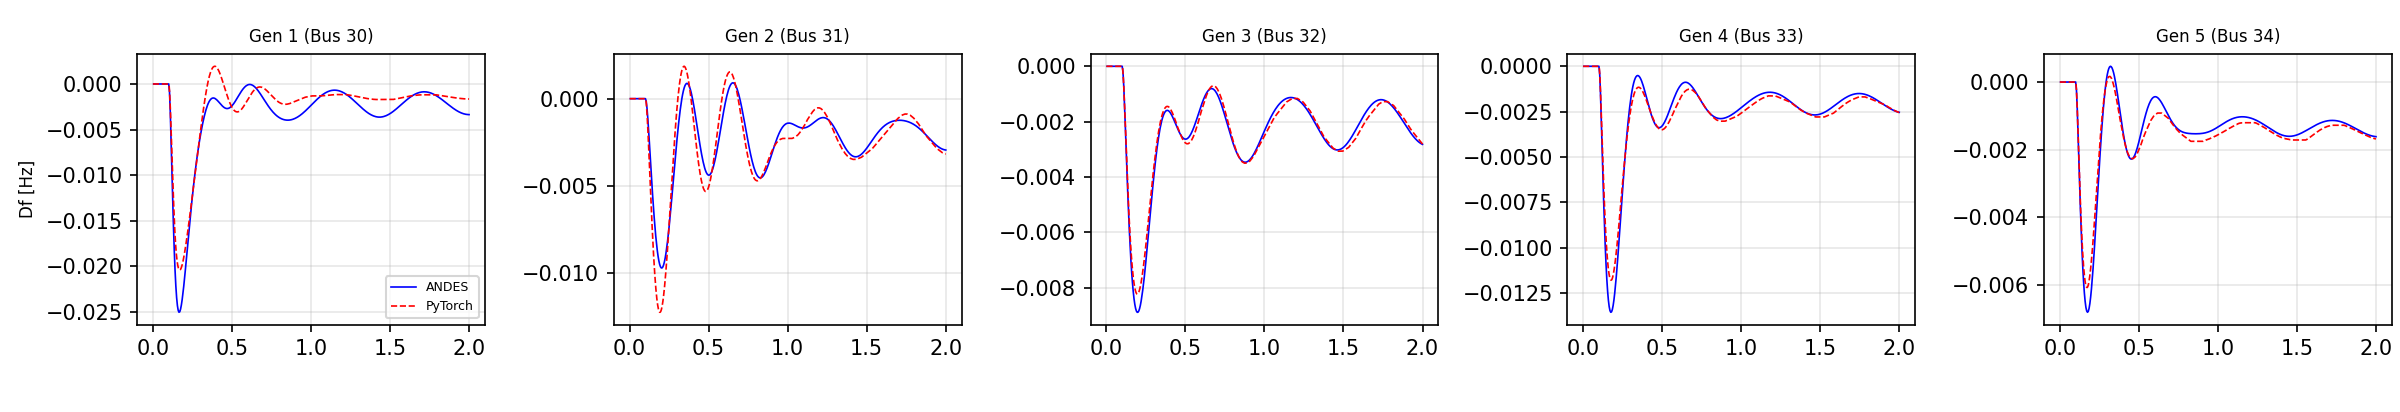
\includegraphics[width=\textwidth]{figures/andes_per_gen_hz_g1g5.png}\\[4pt]
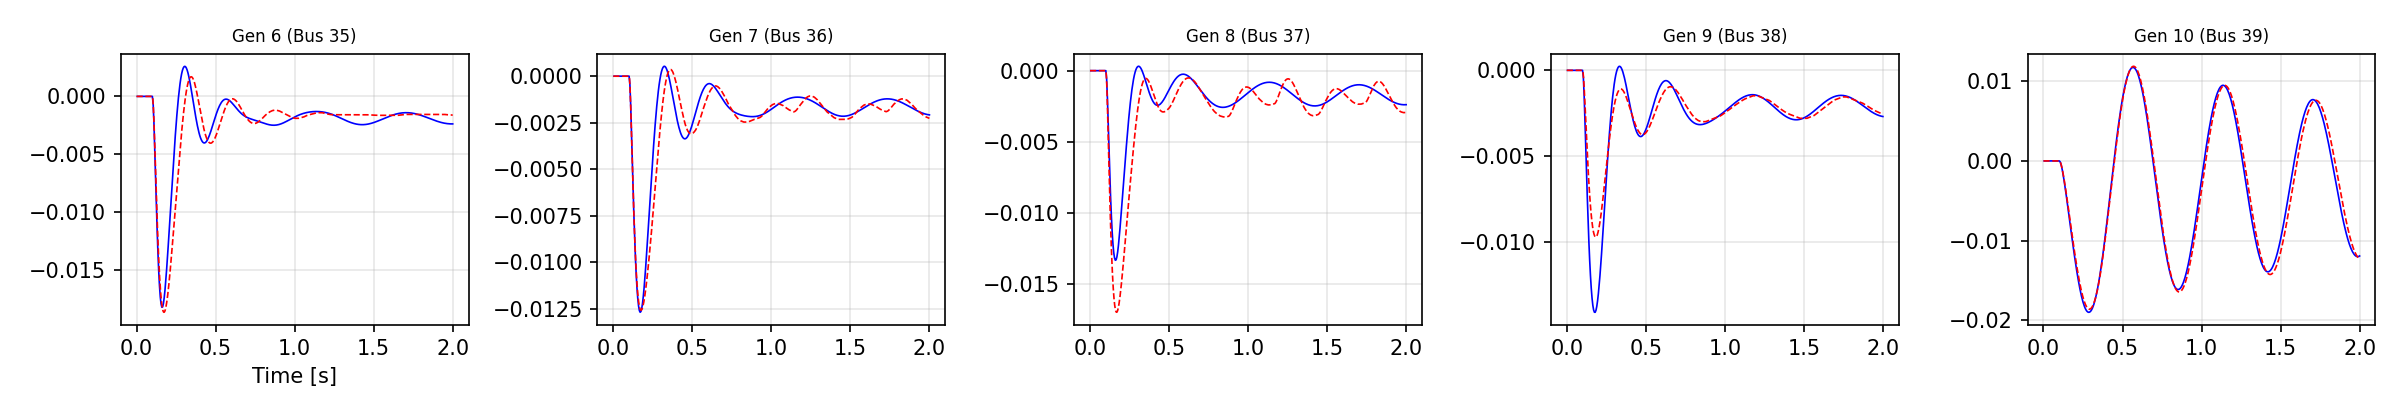
\includegraphics[width=\textwidth]{figures/andes_per_gen_hz_g6g10.png}
\caption{Per-generator frequency comparison: ANDES (blue solid) vs.\
PyTorch (red dashed) under a 200\% load step at bus~18.
Top row: G1--G5; bottom row: G6--G10.}
\label{fig:andes_allgen}
\end{figure*}

Table~\ref{tab:andes_metrics} summarizes per-state-group validation
metrics.  Generator frequency dynamics achieve 0.97 mean correlation
and 0.90~mHz RMS error across all 10 generators.  Mechanical power
and bus voltage dynamics show strong agreement ($>$0.97 and $>$0.84
correlation, respectively).  The worst-case generator nadir difference
(G1: $-25.0$~mHz in ANDES vs.\ $-20.4$~mHz in PyTorch) is consistent
with the 0.83~MW slack-bus dispatch offset redistributing load pickup
among generators through droop control.

\begin{table}[t]
\centering
\caption{ANDES vs.\ PyTorch validation metrics (200\% load step).}
\label{tab:andes_metrics}
\small
\begin{tabular}{lcccc}
\toprule
\textbf{State group} & \textbf{Mean corr.} & \textbf{Min corr.} & \textbf{Mean RMS} & \textbf{Units} \\
\midrule
Gen.\ freq.\ ($\omega$)   & 0.966 & 0.908 & 0.90  & mHz \\
Mech.\ power ($P_m$)      & 0.974 & 0.934 & 0.50  & MW  \\
Bus voltage ($V$)          & 0.840 & 0.768 & 0.025 & pu  \\
Exciter ($E_{fd}$)         & 0.815 & 0.637 & 0.13  & pu  \\
PLL angle ($\phi$)         & 0.915 & 0.841 & 0.13  & rad \\
\bottomrule
\end{tabular}
\end{table}

Fig.~\ref{fig:andes_allgen} shows the per-generator frequency
comparison across all 10 units.  Both simulators capture the same
nadir timing, oscillation period, and recovery envelope.  The residual
per-generator nadir differences (up to 4.6~mHz in mixed directions)
are fully attributable to the documented model-order and
initialization differences, both of which are standard choices in
power systems transient stability analysis~\cite{Kundur94PowerSystems,
SauerPai98}.

\subsection{Training Application}
\label{sec:training}

The differentiable simulator has been used to train neural frequency
controllers for GFM inverter configurations
in~\cite{AlduaijWeng25SGC}.  The
training pipeline uses curriculum learning with gradually increasing
disturbance severity, batched load profiles (32 independent scenarios
per gradient step), and multi-term physics-informed losses including
frequency deviation, RoCoF, control effort, Lyapunov decrease, and ISS
margin penalties.

Table~\ref{tab:training} summarizes the GFM training run.  Over 100
epochs ($\sim$4.8~hours on a single NVIDIA RTX~5080 GPU), the composite
loss converges while the ISS gain bound~$\rho$ decreases from 3.46 to
2.68, indicating improved stability margins.  The per-epoch time
includes 32-sample batched forward simulation (1-second trajectories
at $\Delta t = 1$~ms), IFT backward pass, and Adam optimizer step.
The curriculum gradually increases fault severity, causing temporary
loss increases at mid-training that the controller subsequently
absorbs.

\begin{table}[t]
\centering
\caption{GFM controller training summary (100 epochs, batch size 32).}
\label{tab:training}
\small
\begin{tabular}{lrr}
\toprule
\textbf{Metric} & \textbf{Epoch 0} & \textbf{Epoch 99} \\
\midrule
Composite loss $\mathcal{L}$         & 0.318 & 0.344 \\
Frequency loss $\mathcal{L}_\omega$  & 0.058 & 0.049 \\
RoCoF loss $\mathcal{L}_{\dot\omega}$ & 0.058 & 0.049 \\
ISS gain bound $\rho$                & 3.46  & 2.68  \\
\midrule
Wall-clock time                      & \multicolumn{2}{c}{4.8 hours} \\
Per-epoch time                       & \multicolumn{2}{c}{$\sim$170 s} \\
\bottomrule
\end{tabular}
\end{table}

Because the IFT backward pass provides exact gradients through the
Newton solve at each timestep, the optimizer can train controllers via
standard gradient descent while respecting the DAE constraint
$F(z; x) = 0$.  Without differentiable simulation, the same task
would require gradient-free methods (evolutionary strategies or policy
gradient estimators) with higher sample complexity.

% ============================================================================
\section{Conclusion}
\label{sec:conclusion}
% ============================================================================

This paper presented an open-source, fully differentiable DAE
simulator for the IEEE~39-bus power system with both 6-state
grid-following and 6-state grid-forming inverter models.  The
simulator combines analytic Jacobians for the Newton-based KCL solve
with an implicit function theorem backward pass, providing exact
gradients at computational cost comparable to the forward simulation.

The GFL model has a structural advantage: inverter current injections
depend on differential states (PLL angle, filtered voltage), not on
Newton unknowns, so $\partial I_{\mathrm{inv}}/\partial z = 0$ and
the KCL Jacobian is independent of inverter count.  The GFM model
uses a voltage-behind-impedance interface that couples through the
virtual impedance, adding an admittance diagonal to the Jacobian.
Both models support batched GPU execution, control-affine
decomposition, and incremental energy computation for physics-informed
training.

The simulator has been validated against finite differences for
gradient accuracy and against ANDES for simulation fidelity.  It has
been used to train neural frequency controllers for low-inertia power
systems~\cite{AlduaijWeng25SGC, AlduaijWengLi25BeyondMonotonic},
demonstrating that differentiable simulation enables end-to-end
gradient-based controller optimization on realistic multi-machine
systems.

The codebase is available at \url{https://github.com/halduaij/differentiable-dae-simulator}
under an open-source license.  Future work includes extension to
larger networks (IEEE~118-bus, 2000-bus synthetic grids), integration
of electromagnetic transient (EMT) switching models, and real-time
hardware-in-the-loop deployment.

% ============================================================================
\bibliographystyle{IEEEtran}
\bibliography{ref_arxiv}

\end{document}
